\chapter{Literature Review and Methodology}
\label{chap:review}


CHAPTER SUMMARY

\section{A tale of two particles}

If the reader asks a common person in the street what "electronics" means they will receive a variety of responses centred on computers, smartphones, television sets, and other everyday appliances. On the other hand, if the same interviewee demographic was asked about "photonics", some might mention \acl{led}s (\acs{led}s) and lasers, others might cite Star Trek or other science-fiction work. The term photonics has not found widespread understanding outside the semiconductor industry, despite these two technologies often being separated by around a decade and a half in the research and development stages. 

The basic building block of modern electronics, the transistor, was invented in 1947 \cite{Bardeen1948, Bardeen1950}. Pointing to a direct equivalent in the history of photonics is not straightforward; however, the first solid-state light-emitting device was described just \num{15} years later in 1962 \cite{Biard1966} and consisted of a \acf{gaas} \acs{led} emitting in the infrared. Interest in solid-state lasing grew immediately after this discovery \cite{Hall1962, Hall1963} affirming the role of III-V semiconductors as solid-state light emitters. The next year, in 1963, Wanlass invented \acf{cmos} technology \cite{Wanlass1967} cementing integrated planar electronics as the main computational platform of the second half of the century. It took four years after this seminal invention for the idea of a \acf{pic} to follow \cite{Miller1969}.

Therefore, while integrated electronics was entering its exponential phase, exemplified by Moore's law \cite{Moore1965}, itself formulated in the mid-1960s, the building blocks of photonics were just being discovered or still in a conceptual phase. This led to a difference in investment that, in turn, shaped the technological landscape of humanity. While commercial electron-based technologies were progressing through small-, medium- and large-scale integration, up until very large-scale, photon-based technology was mostly commercialised for, initially highly specialised, lighting and solid-state lasers, until the discovery of the blue \acs{led} in the 1990s \cite{Nakamura1994}. This decade, however, saw a new revolution, the introduction and rapid diffusion of the Internet. This new technology exposed the limitation of the electron as an information-carrying particle. Impedance losses and inductive currents can be sidestepped simply by choosing to transmit information with pulses of light, because fibre optic is much less lossy a support than copper wires, and induction is an issue specific to the electron. This was quite quickly implemented in long-range communication infrastructure, but this technology has been proposed in integrated interconnects since the late 1980s \cite{Miller1989}.

In integrated interconnects, the use of photons bypasses some important problems affecting electrical lines, such as the "aspect ratio limit" that binds the maximum amount of bits per second to the shape of the interconnect \cite{Miller1997}, the dependence of clock timing on temperature, cross-talk between neighbouring interconnects, and the transition between high impedance electronic components and low impedance electronic interconnects, while providing voltage isolation and potential for free space interconnects \cite{Miller1997_reasons}. All of these problems also have electrical solutions, but these solutions in turn increase the energy requirements and therefore the energy loss that occurs on the circuit board, and there is a limit to how much heat can be cost-efficiently extracted from each singular chip; therefore, photonics becomes attractive from both an energy- and a cost-efficiency point of view \cite{Miller2009}, provided that the integration method allows for such an efficiency. 

Indeed, integration is the key step enabling photonics, the initial photonic circuits of the late 1980s and 1990s were realised directly on \acf{inp} wafers from \num{2} inches to \num{4} inches in diameter. Despite the small size, these are very expensive supports compared to the much larger \qty{150}{\milli\metre} and \qty{200}{\milli\metre} \acl{si} supports their contemporary. This technology managed to demonstrate very large scale integration by the mid 2010s, after which it was surpassed by both \acl{si} and III-V on \acl{si} photonic integrated circuits \cite{Shekhar2024, Margalit2021}.

the techs and their properties

\paragraph{\Acl{si} / \acl{si}-\acl{ge} components} unalloyed \acl{si} is mostly used for modulators
\par
\paragraph{\Acl{ge} components}
\par
\paragraph{III-V components}
\par











\section{Properties of III-V materials}

\begin{figure}
    \centering
    \subcaptionbox{
        \hkl{0 0 1} facet.
        \label{subfig:GaAs_100}
    }{
        \tikzsetnextfilename{GaAs_100}
        \begin{tikzpicture}
            \node[inner sep=0pt] (image) at (0, 0) {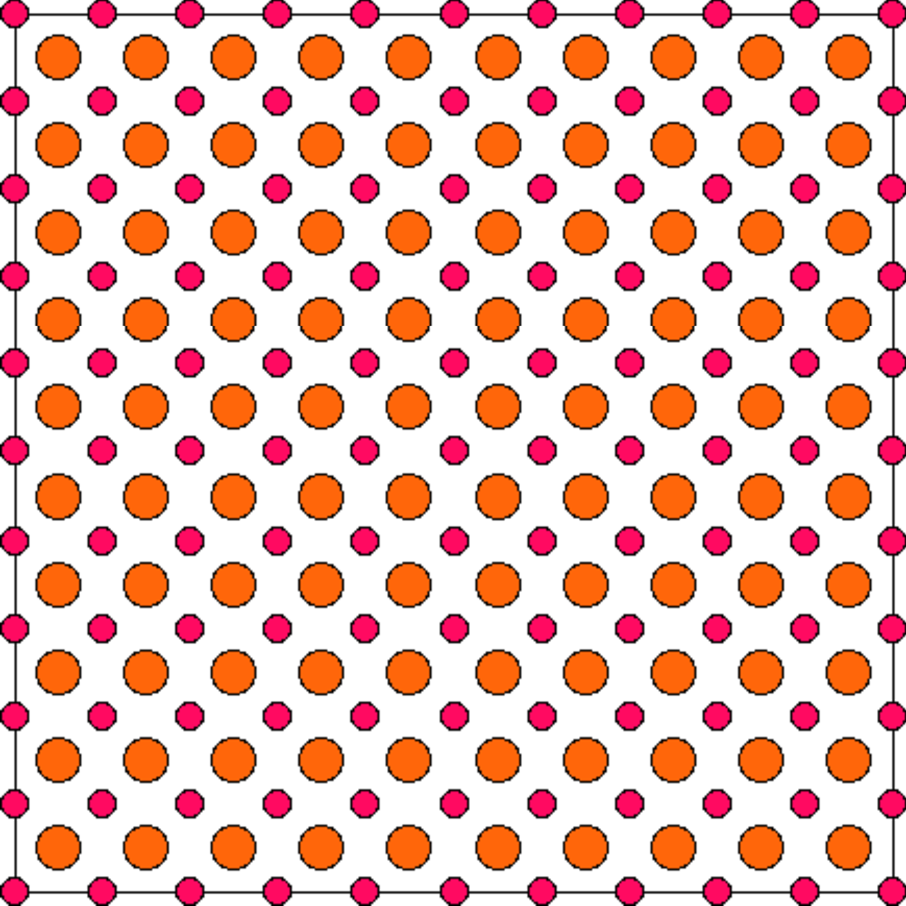
\includegraphics[width=0.30\textwidth]{2_Literature_Review/Fig/GaAs_100.pdf}};
            \draw [fill = black] (0.15, 0.15) rectangle (-0.15, -0.15);
            \draw [white] (0.1, 0.1) -- (-0.1, -0.1);
            \draw [white] (-0.1, 0.1) -- (0.1, -0.1);
        \end{tikzpicture}
    }
    \subcaptionbox{
        \hkl{1 1 0} facet.
        \label{subfig:GaAs_110}
    }{
        \tikzsetnextfilename{GaAs_110}
        \begin{tikzpicture}
            \node[inner sep=0pt] (image) at (0, 0) {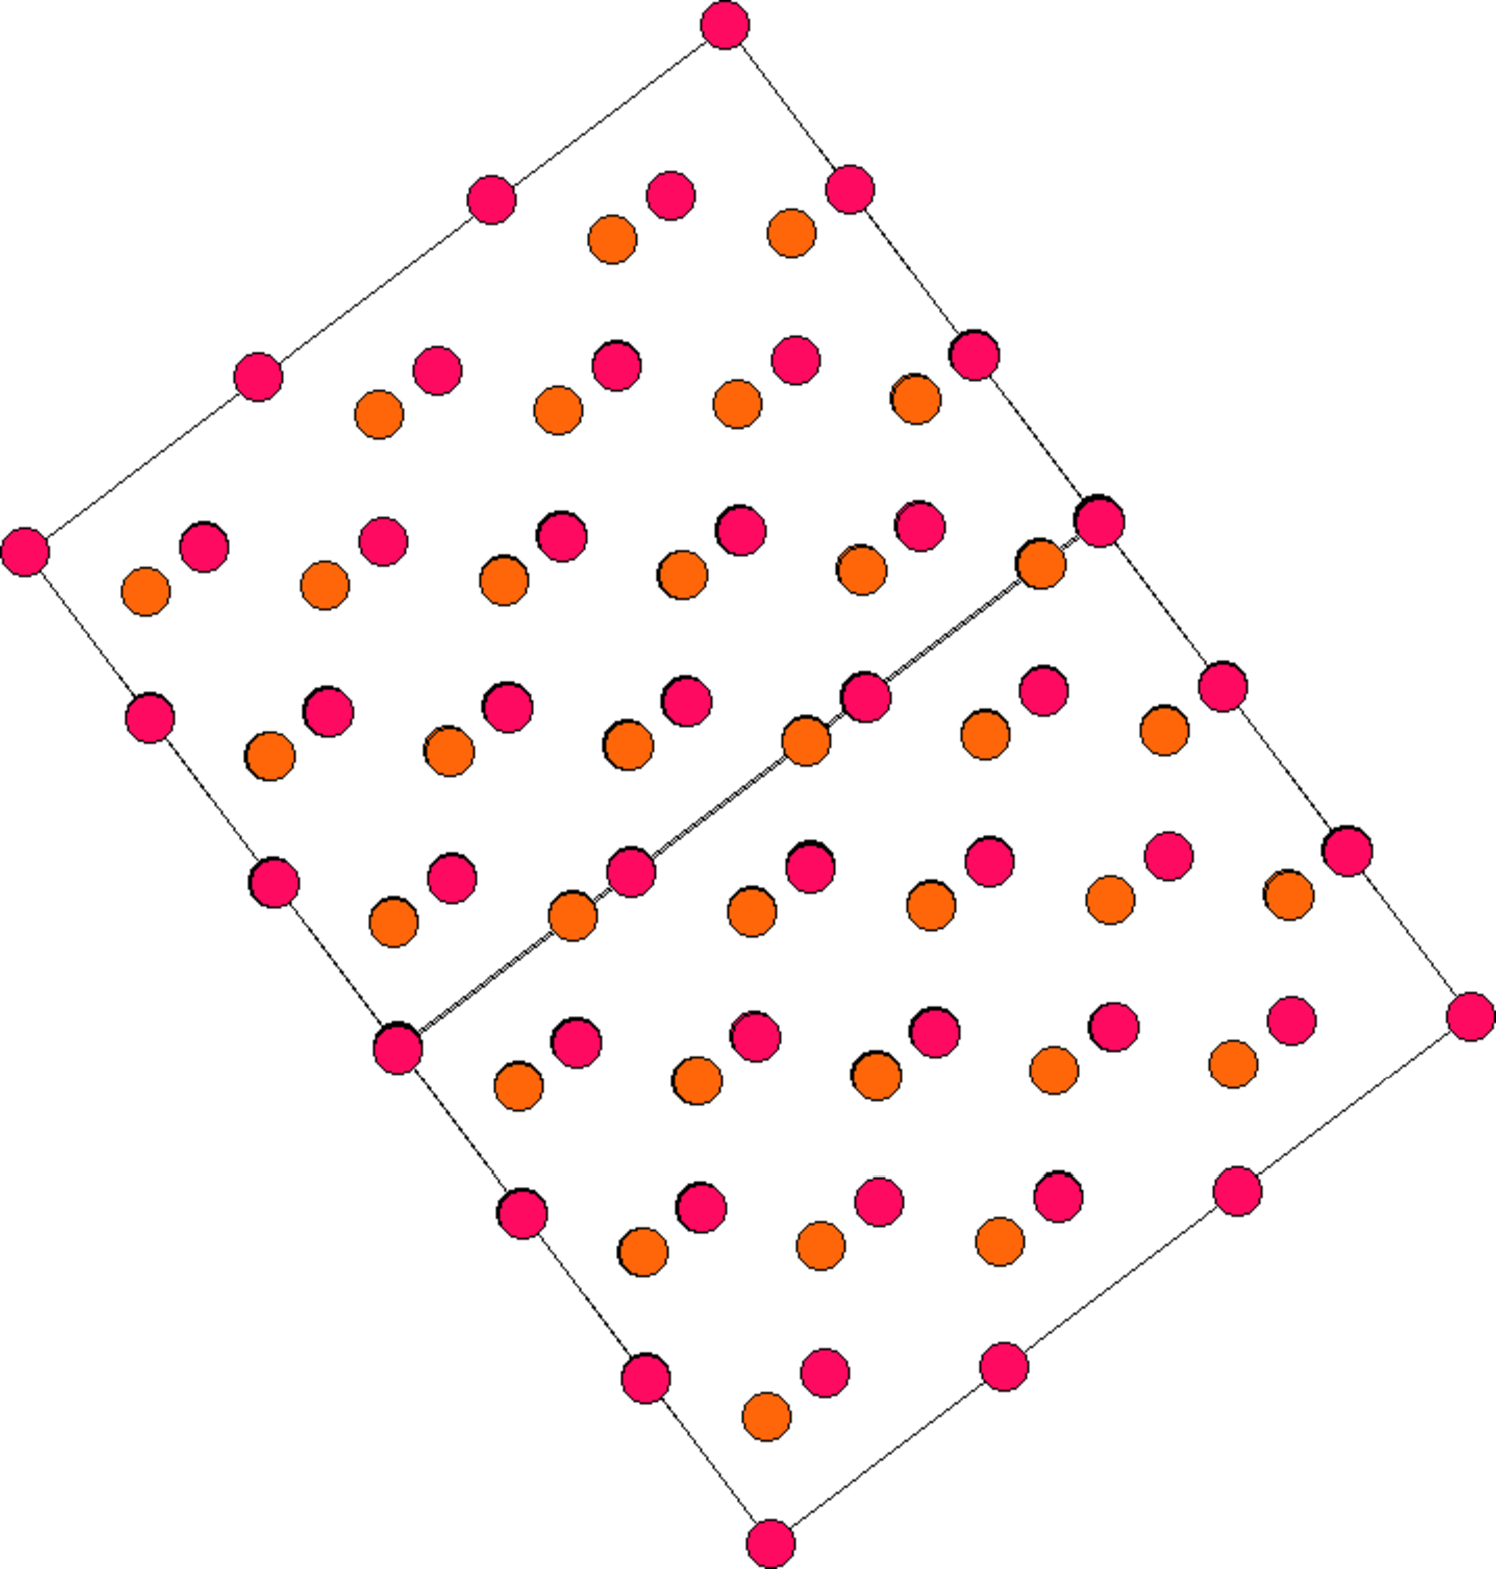
\includegraphics[width=0.30\textwidth]{2_Literature_Review/Fig/GaAs_110.pdf}};
            \begin{scope}[yshift=-0.01]
                \draw (0, 0) -- ++ (37:2);
                \draw (0, 0) -- ++ (37:-2);
                \draw (34:1.9) -- ++ (37:-0.3) -- ++ (-53:0.1) -- cycle;
                \draw (40:1.9) -- ++ (37:-0.3) -- ++ (127:0.1) -- cycle;
            \end{scope}
        \end{tikzpicture}
    }
    \subcaptionbox{
        \hkl{1 1 1}\(_B\) facet.
        \label{subfig:GaAs_111}
    }{
        \tikzsetnextfilename{GaAs_111}
        \begin{tikzpicture}
            \node[inner sep=0pt] (image) at (0, 0) {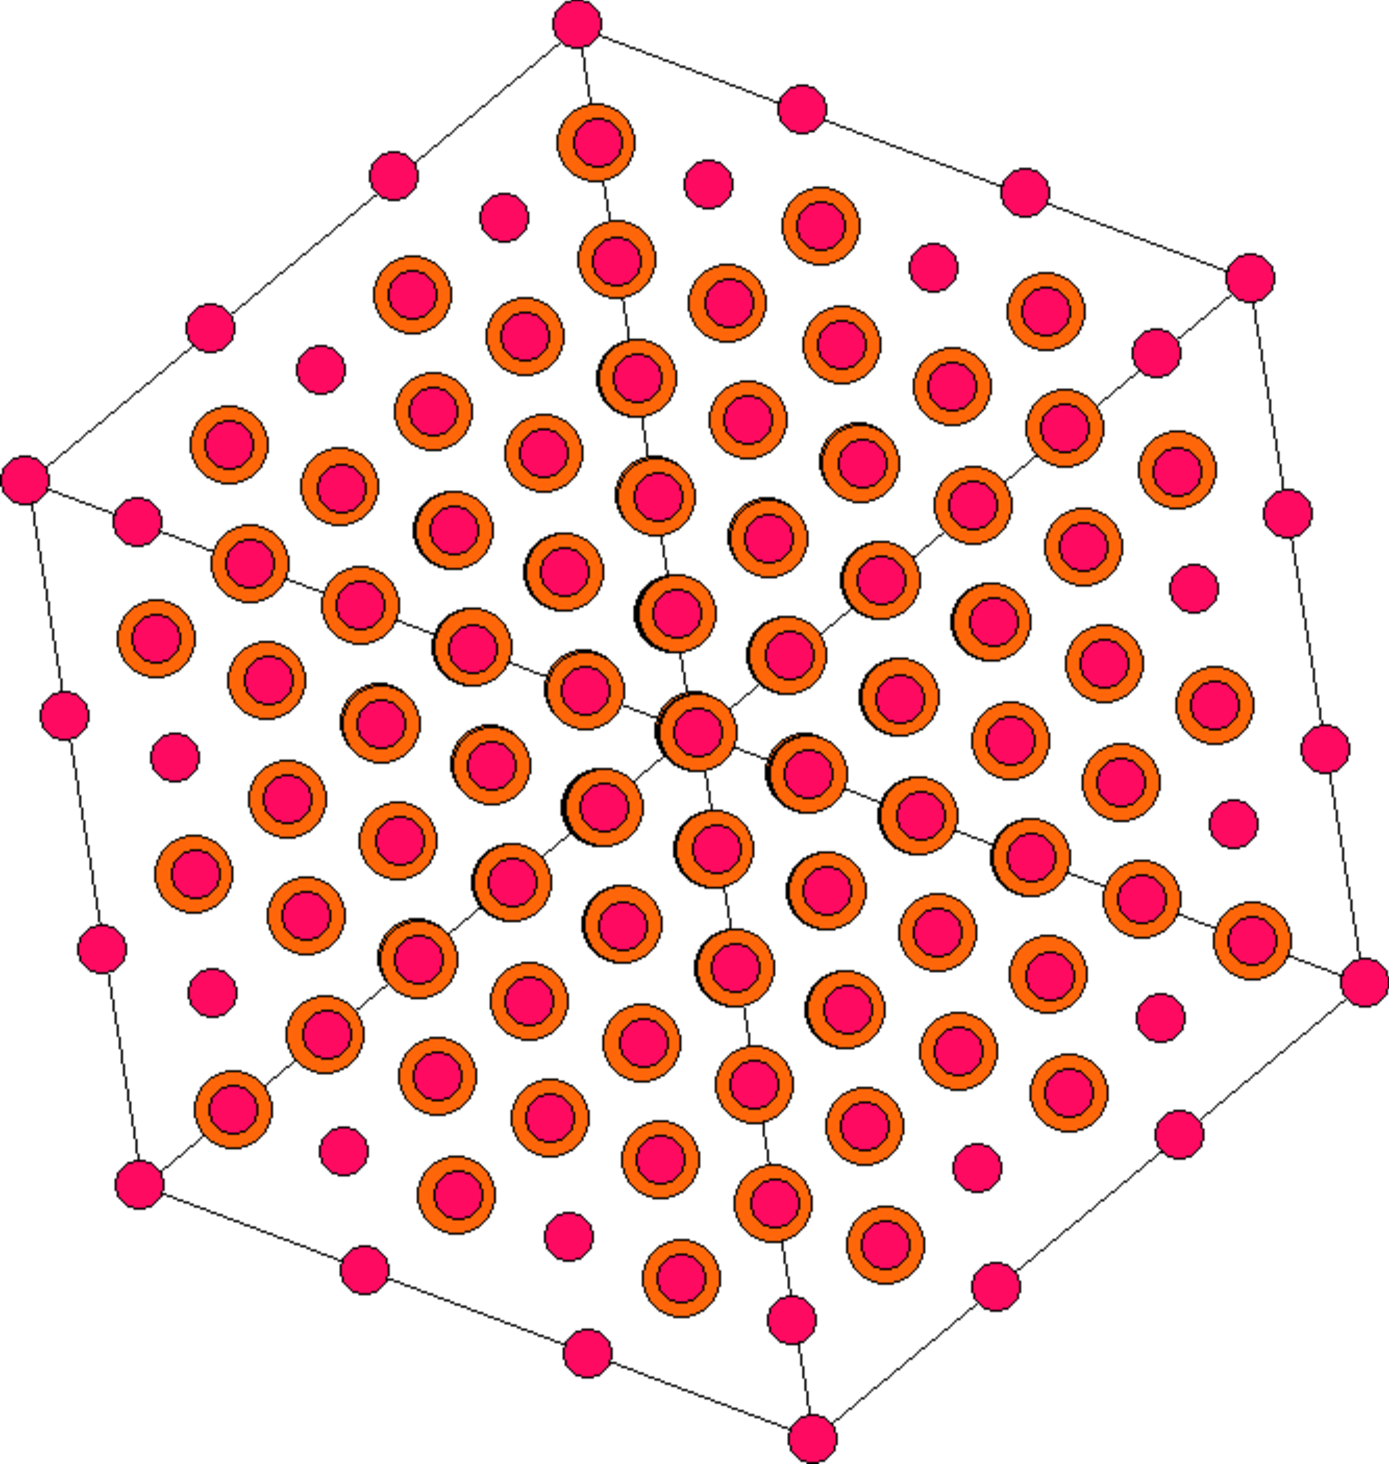
\includegraphics[width=0.30\textwidth]{2_Literature_Review/Fig/GaAs_111.pdf}};
            \draw [fill = black] (0.17, 0) -- ++ (-150:0.3) -- ++ (90:0.3) -- cycle;
            \draw [white] (0, 0) -- ++ (-120:0.1);
            \draw [white] (0, 0) -- ++ (0:0.1);
            \draw [white] (0, 0) -- ++ (120:0.1);
        \end{tikzpicture}
    }
    \caption[Low-index facets in the F-43m \acs{gaas} crystal.]{Simulation of the low-index facets in the F-43m \acs{gaas} crystal with the basic symmetry elements highlighted. \Acl{ga} is represented in orange and \acs{as} in pink; atomic radii are not to scale. \subref{subfig:GaAs_100} shows the 2D projection of the lattice along the \hkl{0 0 1} direction, which coincides with the four-fold axis. \subref{subfig:GaAs_110} shows the 2D projection along the \hkl{1 1 0} direction, contained in the mirror plane. \subref{subfig:GaAs_111} shows the 2D projection along the \hkl{1 1 1} direction, coinciding with the three-fold axis.}
    \label{fig:ZB_low_index_facets}
\end{figure}

III-V semiconductors are compound semiconductors formed by the stoichiometric combination of elements from group III and group V of the periodic table. In their most simple form they are binary, or consisting of one element from group III and one from group V, with some examples being \acs{inp} and \acs{gaas}. Ternary and quaternary III-V materials such as \ce{In1_-_xGa_xAs} or \ce{In1_-_xGa_xAs1_-_yP_y} contain three or four different elements, respectively. 

Crystallographically, III-V materials are available at room temperature in crystals with the symmetries of space group number \num{216} (F-43m, or zincblende-like) or \num{186} (P6\(_3\)mc, or wurtzite-like) and are easily affected by polytypism when grown. Space group \num{216} is that of a cubic face-centred crystal, while space group \num{186} describes a hexagonal crystal. These two structures are closely related, as the addition of a two-fold axis alongside the three-fold axis of space group \num{216} results in a phase change to space group \num{186}, transforming the \hkl<1 1 1> direction in the zincblende phase to the \hkl<0 0 0 1> direction in the wurtzite phase. 











\section{\texorpdfstring{III-V-on-\acs{si} integration routes}{III-V-on-Si integration routes}}
The various integration routes of III-V semiconductors on Si can be divided in two broad categories: heterogeneous and homogeneous integration.
\subsection{Heterogeneous integration}
Heterogeneous integration refers to the indirect integration of III-V material grown on a different, lattice matched, substrate on a Si wafer. 
\par
The main advantage of these techniques is the elimination of lattice mismatch as a source of defects during epitaxial growth. Furthermore, it allows the selection of the best-performing structures to be transferred onto the Si substrate \cite{Zadeh2016, Wang2017}, and does not have to compromise on the growth parameters or material systems for the sake of CMOS compatibility (except for bonding temperature). The various methods that fall under this definition form, all together, a mature technology that already finds application in industry4, therefore benefitting from a few years of industrial optimisation.
\par
On the other hand, this type of integration requires the growth of III-V to take place in a different fabrication line that must maintain the high precision and cleanliness standard of the main CMOS silicon line, resulting in a rather large capital investment. Furthermore, most classic transfer steps can result in a material with a more irregular geometry (wafer bow, surface roughness after etching), or presenting transfer-related defects \cite{Jevtics2022}, or require an extra bonding layer \cite{Jevtics2022, Tang2019}, and do not allow for nm precise integration \cite{Wang2017, McPhillimy2020}. However, the most advanced techniques that bypass most of these quality issues are too slow to provide a competitive transfer time for large, densely integrated 8' production wafers \cite{Wang2017, McPhillimy2020}.
\subsection{Homogeneous Integration}
Homogeneous integration refers to the direct integration by epitaxial growth of III-V semiconductors on Si. 
It naturally provides advantages such as the extremely high spatial precision and accuracy for the integration of small devices on wafer-scale substrates, which can be achieved in a shorter time frame compared to its heterogeneous analogues \cite{Wang2017}. It has the potential of being a more economical alternative to heterogeneous integration. If the growth process can be integrated with current CMOS processes, its implementation in a CMOS line would render having an entire dedicated III-V fab running in parallel with a Si-based fab unnecessary, especially if the use of III-V electronics is envisioned at the same time as III-V photonics \cite{Wang2017}, therefore potentially reducing the capital cost required to implement this efficient light-emitting and -absorbing material in different devices \cite{Tang2019}.
The main disadvantage is related to the high lattice mismatch between Si and most III-V materials, meaning strain-relaxing defects are nucleated at the heterointerface \cite{Kunert2018}: these defects have a very detrimental effect on the performance and lifetime of devices \cite{Mahajan2000, Zenari2021}, and act as scattering or recombination centres \cite{Jeon2015}. The polar nature of III-V atomic bonds compared to nonpolar Si-Si bonds can create anti-phase boundaries during growth on certain Si facets \cite{Kunert2018}, and most known surface treatments to eliminate the nucleation sites for these defects occur in temperature ranges that are incompatible with the CMOS process \cite{Miller2000}. Furthermore, materials that are known to grow at a higher temperature, such as III – nitrides, and others that could have detrimental effects on the passivating of SiO2 layers, such as gallium \cite{Miller2000}, also pose compatibility problems with the CMOS process. Another key obstacle, especially related to the direct growth of micro- and nanostructures, is the stricter requirements for the reproducibility and reliability of the process.
\subsection{Comparison between homogeneous integration routes}
What follows is a table comparing the advantages and disadvantages of various homogeneous integration techniques. The table predominantly focusses on what can be accomplished in the growth reactor and briefly mentions techniques that require simple or complex substrate preparation.


\begin{sidewaystable}
    \centering
\begin{longtable}{p{0.1\textwidth}|p{0.42\textwidth}|p{0.42\textwidth}}
    Type & Advantages & Disadvantages \\ \hline \hline
    Planar growth & 
    \begin{itemize}
        \item Extremely simple substrate preparation steps.
        \item Allows Stranski-Krastanov growth mode for quantum dot formation \cite{Shi2016, Reithmaier2016}
    \end{itemize} & 
    \begin{itemize}
        \item Often leads to wafer bow or warp due to thermal expansion coefficient mismatch \cite{Miyoshi2016, Wang2017_2}
        \item Can require 1+ micrometre thick strain management layer before device growth (depending on mismatch) \cite{Wang2017_2, Cantoro2012}
        \item Widespread defects are common in this kind of growth \cite{Ravash2012}
    \end{itemize} \\ \hline
    Selective Area Growth (SAG) & 
    \begin{itemize}
        \item Substrate preparation ranges from relatively simple to somewhat complex
        \item Allows the growth of nanostructures \cite{Cantoro2012}
        \item Allows the growth of core-shell wires \cite{Tomioka2011}
        \item Allows position control \cite{Tomioka2011}
        \item No wafer warp or bow as a result of the III-V material
        \item Allows the growth of various device structures, but only vertically \cite{Bi2019, Staudinger2021}
    \end{itemize}  & 
    \begin{itemize}
        \item Sidewall growth can be minimized but not eliminated, resulting in undesired heterointerfaces and possible loss of composition control in complex systems.
        \item Growth mainly happens in the vertical direction
    \end{itemize}  \\ \hline
    VLS/Droplet epitaxy (vertical nanowires) & 
    \begin{itemize}
        \item Simple substrate preparation process
        \item Allows for nanostructure growth \cite{Wagner1964}
        \item No wafer warp or bow as a result of the III-V material
        \item Allows for sophisticated growth studies such as in-situ TEM imaging \cite{Maliakkal2020, Jacobsson2016, Harmand2018}, leading to the possibility to refine growth recipes to the point where phase control can be achieved \cite{Algra2008, Caroff2009, Joyce2007}.
        \item Can be tuned to achieve high directionality of the growth and possibility to incorporate heterostructures with minimal or no undesired side growth \cite{Harmand2018, Joyce2007}
    \end{itemize}  & \begin{itemize}
        \item Limited position control \cite{Joyce2007}
        \item Nanostructure geometry limited to nanowires \cite{Wagner1964}
        \item Reservoir effect complicates composition control in ternary and quaternary compounds \cite{Dubrovskii2017}
    \end{itemize} \\ \hline
    \caption{Caption}
    \label{tab:methods1}
\end{longtable}
\end{sidewaystable}
    \begin{sidewaystable}
    \centering
    \begin{longtable}{p{0.1\textwidth}|p{0.42\textwidth}|p{0.42\textwidth}}
    Type & Advantages & Disadvantages \\ \hline \hline
    Selective Area Growth with Aspect Ratio Trapping & 
    \begin{itemize}
        \item Allows position control for the III-V growth29
        \item Highly reduced bow and warp effect on the wafer after deposition
        \item Aspect ratio trapping (ART) allows a base level of defect control \cite{Han2016}
    \end{itemize}  & \begin{itemize}
        \item Defects propagating in any direction that shares the plane of the side walls are not filtered2
        \item Multiple nucleation points can result in grain boundaries, and their elimination requires extra process steps \cite{Kunert2016}
    \end{itemize} \\ \hline
    Template Assisted Selective Epitaxy (TASE) & 
    \begin{itemize}
        \item Allows the growth of a very large variety of both vertical and horizontal nanostructures while maintaining extremely accurate geometry and  position control \cite{Ritter2021, Tiwari2020, Schmid2015}
        \item Superior defect control, even compared with ART: far from the growth interface defects can be effectively limited to twin planes \cite{Han2020}, which in some cases can too be eliminated \cite{Knoedler2017}
        \item Potential for excellent facet and composition \cite{Borg2019, Goswami2020} control in nanowires, with no side growth when growing heterostructures \cite{Brunelli2019} 
        \item No wafer warp or bow as a result of the III-V material
        \item Allows for phase control in determinate growth geometries \cite{Staudinger2018}
    \end{itemize} & 
    \begin{itemize}
        \item Substrate preparation takes place in a complex multi-step process
        \item Can suffer from parasitic growth
        \item Some height limitations in terms of core shell structures, which can’t be grown horizontally, and are de-facto limited to microdisk form factors \cite{Tiwari2020}
    \end{itemize} \\ \hline
    \caption{Caption}
    \label{tab:methods2}
\end{longtable}
\end{sidewaystable}

It should be noted that often, in papers from Dr. Lau’s group, the growth method they use is called lateral aspect ratio trapping (LART) \cite{Han2020, Yan2021}: this is in essence a hybrid between SAG-ART and TASE, and can be described as a type of TASE with particularly wide (sometimes several micrometres) templates, therefore I have grouped it with TASE in the above table. It should be noted, however, that while LART offers most of the same advantages that TASE offers, it is more susceptible to the formation of grain boundaries due to multiple nucleation (which does not take place in TASE) and has reduced defect trapping in the wide direction. On the other hand, due to their etch-based approach, they can achieve more intricate quantum well positioning in their microdisk lasers than what is possible with our TASE approach for microdisk growth.



111B growth outside of tase

\section{\texorpdfstring{State of \acl{tase}}{State of template assisted selective epitaxy}}
\section{Characterization of nano- and microstructures}
Talk about defect types (what is an rtp is very important) and therefore about the lattices

TALK ABOUT IMPORTANCE OF SINGLE FACET FOR INCORPORATION RATES (SEE FOLLOWING SECTION)

\section{Article 2}

Due to the presence of the SiO2 template, the quantum wells
develop only axially and not laterally. This results in improved
composition control in heterolayers of ternary III-V
compounds incorporated in the nanowires\cite{Borg2019} and therefore is
expected to allow for better control of the emission spectra.